\section{Three 4-transpositions}

\begin{lemma}
  If $\rho_0$ is a 2-transposition then there must be a single $\rho_1$ edge (and thus a single $\rho_3$ edge).
\end{lemma}

\begin{proof}
  By Lemma~\ref{adjacent-must-not-commute}, a $\rho_0$ must be adjacent to a $\rho_1$ edge. The $\rho_1$ can be a single edge, a double edge with another involution or on an alternating square.

  \paragraph{}
  If the $\rho_1$ edge is on a double edge then this edge can be $\rho_2$ or $\rho_3$. But the if $\rho_0$ and $\rho_1$ does not commute in this location~\footnote{...} then $\rho_0$ does not commute with the other involution and this is a contradiction with Proposition~\ref{intersection-patterns}.

  \paragraph{}
  If $\rho_1$ is on an alternating square, the same occurs\footnote{to do}.

\end{proof}

\begin{lemma}
  There cannot be more than one $\rho_1$ single edge and thus there cannot be more than one $\rho_3$ single edge.
\end{lemma}

\begin{proof}
  There are not enough points otherwise.
\end{proof}

\begin{corollary}
  \label{rank-4-single-1}
  If $\rho_0$ is a 2-transposition then there is exactly one $\rho_1$ single edge and one $\rho_3$ single edge.
\end{corollary}

\begin{lemma}
  \label{rank-4-3-patterns}
  Let $\Gamma$ be a sggi of rank 4 on 11 points. If $\rho_1$, $\rho_2$ and $\rho_3$ are 4-transpositions and $\rho_0$ is a 2-transposition then the patterns formed by $\rho_1$ and $\rho_3$ edges are one alternating square, one double edge and two simple edges (one for each involution).\footnote{Extend this part}
\end{lemma}

\begin{proof}
  By Corollary~\ref{rank-4-single-1} there are exactly one $\rho_1$ single edge. The remaining possibilities for the three remaining edges are limited: one alternating square $[\rho_1, \rho_3]$ and one double edge $(\rho_1, \rho_3)$ or three double edges $(\rho_1, \rho_3)$.

  \paragraph{}
  Suppose that there are three double edges.

    \begin{figure}[H]
      \begin{center}
        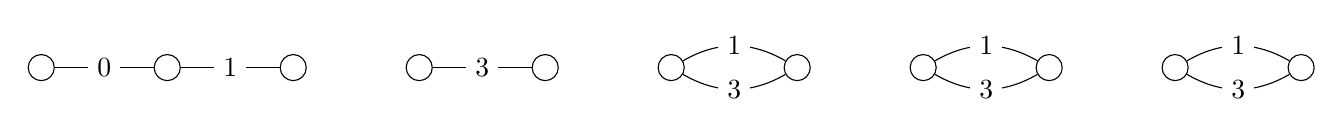
\begin{tikzpicture}[scale=.8]

          \begin{scope}[every node/.style={circle,draw}]
            \node (1)  at (0,0)  {};
            \node (2)  at (2,0)  {};
            \node (3)  at (4,0)  {};
            \node (4)  at (6,0) {};
            \node (5)  at (8,0)  {};
            \node (6)  at (10,0)  {};
            \node (7)  at (12,0)  {};
            \node (8)  at (14,0)  {};
            \node (9)  at (16,0)  {};
            \node (10) at (18,0)  {};
            \node (11) at (20,0)  {};
          \end{scope}

          \begin{scope}[every node/.style={fill=white}]

            \begin{scope}[every edge/.style={draw}]
              \path (1)  edge node {$0$} (2);
              \path (2)  edge node {$1$} (3);
              \path (6)  edge[bend left=30] node {$1$} (7);
              \path (8)  edge[bend left=30] node {$1$} (9);
              \path (10) edge[bend left=30] node {$1$} (11);
              \path (4)  edge node {$3$} (5);
              \path (6)  edge[bend right=30] node {$3$} (7);
              \path (8)  edge[bend right=30] node {$3$} (9);
              \path (10) edge[bend right=30] node {$3$} (11);
            \end{scope}
          \end{scope}

        \end{tikzpicture}
        \caption{}
      \end{center}
    \end{figure}

  \paragraph{}
  But now by~\ref{todo}\footnote{Not complete}, we can clearly see that the other $\rho_0$ edge will never be placed.
\end{proof}

\begin{theorem}
  All sggi of rank 4 on $A_{11}$ with three 4-transpositions are those displayed in appendix~\ref{rank4-3-4transpositions}
\end{theorem}

\begin{proof}
  Let, without loss of generality, $\rho_1$ and $\rho_3$ be 4-transposition.

  \begin{figure}[H]
    \begin{center}
      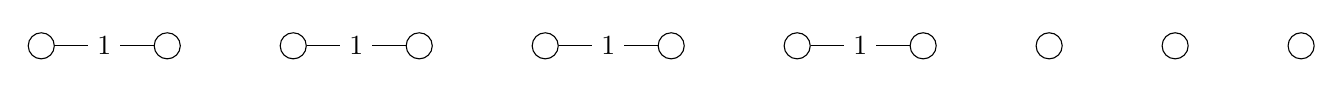
\begin{tikzpicture}[scale=.8]

        \begin{scope}[every node/.style={circle,draw}]
          \node (1)  at (0,0)  {};
          \node (2)  at (2,0)  {};
          \node (3)  at (4,0)  {};
          \node (4)  at (6,0)  {};
          \node (5)  at (8,0)  {};
          \node (6)  at (10,0)  {};
          \node (7)  at (12,0)  {};
          \node (8)  at (14,0)  {};
          \node (9)  at (16,0)  {};
          \node (10) at (18,0)  {};
          \node (11) at (20,0) {};
        \end{scope}

        \begin{scope}[every node/.style={fill=white}]

          \begin{scope}[every edge/.style={draw}]
            \path (1)  edge node {$1$} (2);
            \path (3)  edge node {$1$} (4);
            \path (5)  edge node {$1$} (6);
            \path (7)  edge node {$1$} (8);
          \end{scope}
        \end{scope}

      \end{tikzpicture}
      \caption{}
    \end{center}
  \end{figure}

  \paragraph{}By Lemma~\ref{rank-4-3-patterns}, the pattern between $\rho_1$ and $\rho_3$ is the following.


  \begin{figure}[H]
    \begin{center}
      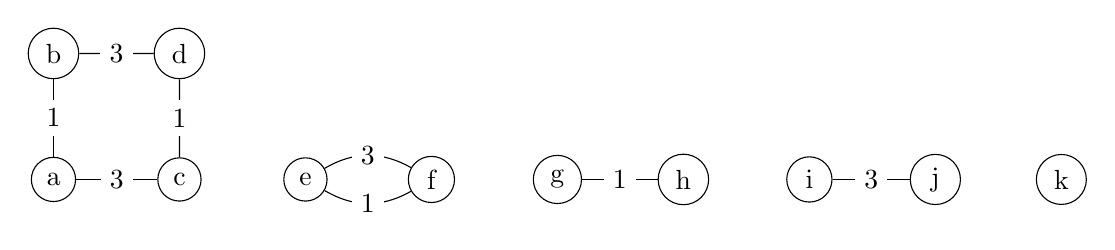
\begin{tikzpicture}[scale=.8]

        \begin{scope}[every node/.style={circle,draw}]
          \node (1)  at (0,2)  {b};
          \node (2)  at (0,0)  {a};
          \node (3)  at (2,2)  {d};
          \node (4)  at (2,0)  {c};
          \node (5)  at (4,0)  {e};
          \node (6)  at (6,0)  {f};
          \node (7)  at (8,0)  {g};
          \node (8)  at (10,0) {h};
          \node (9)  at (12,0) {i};
          \node (10) at (14,0) {j};
          \node (11) at (16,0) {k};
        \end{scope}

        \begin{scope}[every node/.style={fill=white}]

          \begin{scope}[every edge/.style={draw}]
            \path (1)  edge node {$1$} (2);
            \path (3)  edge node {$1$} (4);
            \path (5)  edge[bend right=30] node {$1$} (6);
            \path (7)  edge node {$1$} (8);
            \path (1)  edge node {$3$} (3);
            \path (2)  edge node {$3$} (4);
            \path (5)  edge[bend left=30] node {$3$} (6);
            \path (9)  edge node {$3$} (10);
          \end{scope}
        \end{scope}

      \end{tikzpicture}
      \caption{}
    \end{center}
  \end{figure}

  \paragraph{}
  We will used our notion of "joker" edges. In this case there are 14 edges to link 11 vertices. Thus we have 4 "joker" edges. But two of them have already been used to build the alternating square and the double edge.

  \paragraph{}
  Let's place the $\rho_0$ edges. We know by the proof of the previous lemma that one edge must be adjacent to the single $\rho_1$ edge.

  \begin{figure}[H]
    \begin{center}
      \begin{tikzpicture}[scale=.8]

        \begin{scope}[every node/.style={circle,draw}]
          \node (1)  at (0,2)  {};
          \node (2)  at (0,0)  {};
          \node (3)  at (2,2)  {};
          \node (4)  at (2,0)  {};
          \node (5)  at (4,0)  {};
          \node (6)  at (6,0)  {};
          \node (7)  at (14,0)  {};
          \node (8)  at (12,0)  {};
          \node (9)  at (8,0)  {};
          \node (10) at (10,0)  {};
          \node (11) at (16,0) {};
        \end{scope}

        \begin{scope}[every node/.style={fill=white}]

          \begin{scope}[every edge/.style={draw}]
            \path (7)  edge node {$0$} (11);
            \path (1)  edge node {$1$} (2);
            \path (3)  edge node {$1$} (4);
            \path (5)  edge[bend left=30] node {$1$} (6);
            \path (7)  edge node {$1$} (8);
            \path (1)  edge node {$3$} (3);
            \path (2)  edge node {$3$} (4);
            \path (5)  edge[bend right=30] node {$3$} (6);
            \path (9)  edge node {$3$} (10);
          \end{scope}
        \end{scope}

      \end{tikzpicture}
      \caption{}
    \end{center}
  \end{figure}

  \paragraph{}The other $\rho_0$ cannot connect different components\footnote{Justify}. Furthermore it cannot be used in the component $\{i,j,k\}$. If it is used in the component $\{e,f\}$ Then this component must be part of an alternating square. But the only available involution to make this alternating square is $\rho_2$. But then this new component cannot be linked by $\rho_2$ edges\footnote{Graph}.

  \paragraph{}
  Thus the last $\rho_0$ edge must be used in the $\{a,b,c,d\}$ component.

  \begin{figure}[H]
    \begin{center}
      \begin{tikzpicture}[scale=.8]

        \begin{scope}[every node/.style={circle,draw}]
          \node (1)  at (0,2)  {};
          \node (2)  at (0,0)  {};
          \node (3)  at (2,2)  {};
          \node (4)  at (2,0)  {};
          \node (5)  at (4,0)  {};
          \node (6)  at (6,0)  {};
          \node (7)  at (14,0)  {};
          \node (8)  at (12,0)  {};
          \node (9)  at (8,0)  {};
          \node (10) at (10,0)  {};
          \node (11) at (16,0) {};
        \end{scope}

        \begin{scope}[every node/.style={fill=white}]

          \begin{scope}[every edge/.style={draw}]
            \path (1)  edge[bend left=30] node {$0$} (3);
            \path (7)  edge node {$0$} (11);
            \path (1)  edge node {$1$} (2);
            \path (3)  edge node {$1$} (4);
            \path (5)  edge[bend left=30] node {$1$} (6);
            \path (7)  edge node {$1$} (8);
            \path (1)  edge[bend right=30] node {$3$} (3);
            \path (2)  edge node {$3$} (4);
            \path (5)  edge[bend right=30] node {$3$} (6);
            \path (9)  edge node {$3$} (10);
          \end{scope}
        \end{scope}

      \end{tikzpicture}
      \caption{}
    \end{center}
  \end{figure}

  \paragraph{}
  There are only 4 $\rho_2$ edges to be placed. Three of them must link the components because there are only on "joker" edge remaining. There are multiple way to link those components. As for the previous section, all the permutation representation graphs are diplayed in Appendix~\ref{rank4-3-4transpositions}. We only consider one graph but the reader can check that all the following statement can be applied to all other variants.

  \begin{figure}[H]
    \begin{center}
      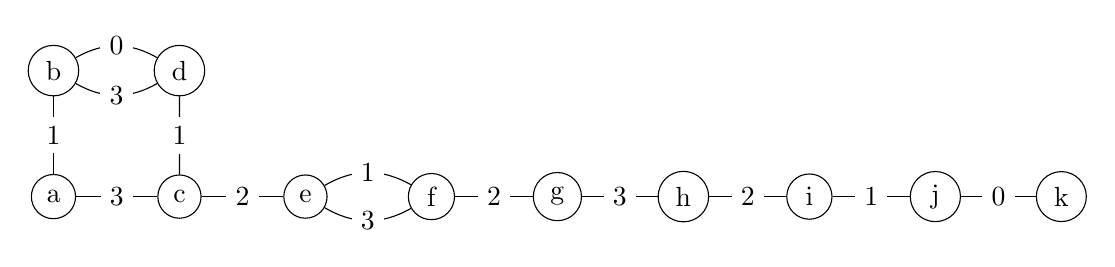
\begin{tikzpicture}[scale=.8]

        \begin{scope}[every node/.style={circle,draw}]
          \node (1)  at (0,2)  {b};
          \node (2)  at (0,0)  {a};
          \node (3)  at (2,2)  {d};
          \node (4)  at (2,0)  {c};
          \node (5)  at (4,0)  {e};
          \node (6)  at (6,0)  {f};
          \node (7)  at (14,0)  {j};
          \node (8)  at (12,0)  {i};
          \node (9)  at (8,0)  {g};
          \node (10) at (10,0)  {h};
          \node (11) at (16,0) {k};
        \end{scope}

        \begin{scope}[every node/.style={fill=white}]

          \begin{scope}[every edge/.style={draw}]
            \path (1)  edge[bend left=30] node {$0$} (3);
            \path (7)  edge node {$0$} (11);
            \path (1)  edge node {$1$} (2);
            \path (3)  edge node {$1$} (4);
            \path (5)  edge[bend left=30] node {$1$} (6);
            \path (7)  edge node {$1$} (8);
            \path (4)  edge node {$2$} (5);
            \path (6)  edge node {$2$} (9);
            \path (10) edge node {$2$} (8);
            \path (1)  edge[bend right=30] node {$3$} (3);
            \path (2)  edge node {$3$} (4);
            \path (5)  edge[bend right=30] node {$3$} (6);
            \path (9)  edge node {$3$} (10);
          \end{scope}
        \end{scope}

      \end{tikzpicture}
      \caption{}
    \end{center}
  \end{figure}

  \paragraph{}
  The last $\rho_2$ edge one must double something. The only two possibilities: triple the double edge $(b, d)$ or double the edge $(j,k)$.

  \paragraph{}
  If the edge $(j,k)$ is doubled, the graph is the following.

  \begin{figure}[H]
    \begin{center}
      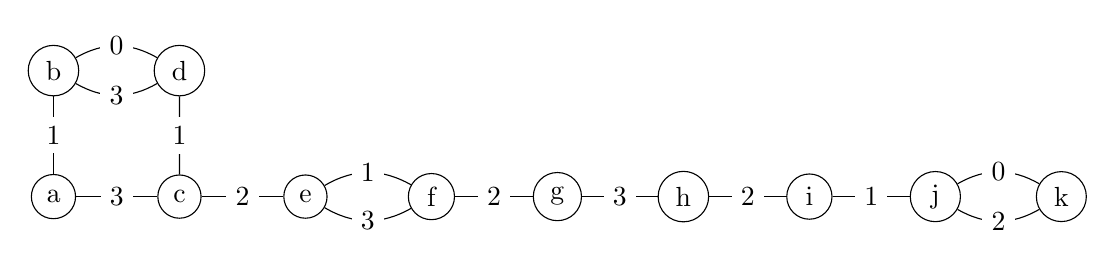
\begin{tikzpicture}[scale=.8]

        \begin{scope}[every node/.style={circle,draw}]
          \node (1)  at (0,2)  {b};
          \node (2)  at (0,0)  {a};
          \node (3)  at (2,2)  {d};
          \node (4)  at (2,0)  {c};
          \node (5)  at (4,0)  {e};
          \node (6)  at (6,0)  {f};
          \node (7)  at (14,0)  {j};
          \node (8)  at (12,0)  {i};
          \node (9)  at (8,0)  {g};
          \node (10) at (10,0)  {h};
          \node (11) at (16,0) {k};
        \end{scope}

        \begin{scope}[every node/.style={fill=white}]

          \begin{scope}[every edge/.style={draw}]
            \path (1)  edge[bend left=30] node {$0$} (3);
            \path (7)  edge[bend left=30] node {$0$} (11);
            \path (1)  edge node {$1$} (2);
            \path (3)  edge node {$1$} (4);
            \path (5)  edge[bend left=30] node {$1$} (6);
            \path (7)  edge node {$1$} (8);
            \path (4)  edge node {$2$} (5);
            \path (6)  edge node {$2$} (9);
            \path (10) edge node {$2$} (8);
            \path (7) edge[bend right=30] node {$2$} (11);
            \path (1)  edge[bend right=30] node {$3$} (3);
            \path (2)  edge node {$3$} (4);
            \path (5)  edge[bend right=30] node {$3$} (6);
            \path (9)  edge node {$3$} (10);
          \end{scope}
        \end{scope}

      \end{tikzpicture}
      \caption{}
    \end{center}
  \end{figure}

  \paragraph{}
  If the $\rho_1$ edge is removed the graph this one (for every variation too):

  \begin{figure}[H]
    \begin{center}
      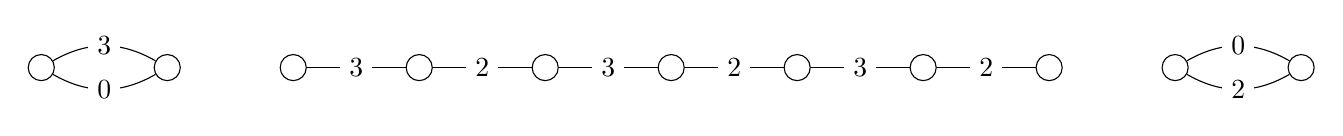
\begin{tikzpicture}[scale=.8]

        \begin{scope}[every node/.style={circle,draw}]
          \node (1)  at (-4,0)  {};
          \node (2)  at (-2,0)  {};
          \node (3)  at (14,0)  {};
          \node (4)  at (16,0) {};
          \node (5)  at (8,0)  {};
          \node (6)  at (10,0)  {};
          \node (7)  at (0,0)  {};
          \node (8)  at (2,0)  {};
          \node (9)  at (4,0)  {};
          \node (10) at (6,0)  {};
          \node (11) at (12,0)  {};
        \end{scope}

        \begin{scope}[every node/.style={fill=white}]

          \begin{scope}[every edge/.style={draw}]
            \path (1)  edge[bend right=30] node {$0$} (2);
            \path (3)  edge[bend left=30] node {$0$} (4);
            \path (3)  edge[bend right=30] node {$2$} (4);
            \path (5)  edge node {$2$} (10);
            \path (6)  edge node {$2$} (11);
            \path (8)  edge node {$2$} (9);
            \path (1)  edge[bend left=30] node {$3$} (2);
            \path (5)  edge node {$3$} (6);
            \path (7)  edge node {$3$} (8);
            \path (9)  edge node {$3$} (10);
          \end{scope}
        \end{scope}

      \end{tikzpicture}
      \caption{}
    \end{center}
  \end{figure}

  \paragraph{}
  But here it is clear that $\rho_0 = (\rho_2 \rho_3)^7$. Thus the last $\rho_2$ edge must triple to existing double edge. Therefore the last $\rho_2$ edge must be $(b,d)$.

  \begin{figure}[H]
    \begin{center}
      \begin{tikzpicture}[scale=.8]

        \begin{scope}[every node/.style={circle,draw}]
          \node (1)  at (2,2)  {};
          \node (2)  at (0,2)  {};
          \node (3)  at (14,0)  {};
          \node (4)  at (16,0) {};
          \node (5)  at (8,0)  {};
          \node (6)  at (10,0)  {};
          \node (7)  at (0,0)  {};
          \node (8)  at (2,0)  {};
          \node (9)  at (4,0)  {};
          \node (10) at (6,0)  {};
          \node (11) at (12,0)  {};
        \end{scope}

        \begin{scope}[every node/.style={fill=white}]

          \begin{scope}[every edge/.style={draw}]
            \path (1)  edge[bend right=45] node {$0$} (2);
            \path (3)  edge node {$0$} (4);
            \path (1)  edge node {$1$} (8);
            \path (2)  edge node {$1$} (7);
            \path (3)  edge node {$1$} (11);
            \path (9)  edge[bend left=30] node {$1$} (10);
            \path (1)  edge node {$2$} (2);
            \path (5)  edge node {$2$} (10);
            \path (6)  edge node {$2$} (11);
            \path (8)  edge node {$2$} (9);
            \path (1)  edge[bend left=45] node {$3$} (2);
            \path (5)  edge node {$3$} (6);
            \path (7)  edge node {$3$} (8);
            \path (9)  edge[bend right=30] node {$3$} (10);
          \end{scope}
        \end{scope}

      \end{tikzpicture}
      \caption{}
    \end{center}
  \end{figure}

\end{proof}

\begin{theorem}
  None of those graphs are C-groups.
\end{theorem}

\begin{proof}
  As for previous similar proof, only the summary is displayed and the details is left to the reader.

  \begin{table}[H]
    \centering
    \begin{tabular}{|c|c|c|c|c|c|c|}
      \hline
      Figure & $\Gamma_3$ & $\Gamma_0$ & $\Gamma_{0,3}$ & $\#\Gamma_{0,3}$ & $\Gamma_3 \cap \Gamma_0$ & $\#(\Gamma_3 \cap \Gamma_0)$ \\ \hline

      \ref{r4-5-1} & $S_7 : D_8$ & $A_{10}$ & $D_{42}$ & 42 & $\ge S_5$ & $\ge 120$ \\ \hline
      \ref{r4-5-2} & $A_{10}$ & $A_{10}$ & $D_{18}$ & 18 & $A_9$ & $181440$ \\ \hline
      \ref{r4-5-3} & $A_{10}$ & $A_{10}$ & $D_{18}$ & 18 & $A_9$ & $181440$ \\ \hline
      \ref{r4-5-4} & $S_7 : D_8$ & $A_{10}$ & $D_{42}$ & 42 & $\ge S_5$ & $\ge 120$ \\ \hline
      \ref{r4-5-5} & $A_5 : S_6$ & $A_{10}$ & $D_{10}$ & 10 & $\ge S_4$ & $\ge 24$ \\ \hline
      \ref{r4-5-6} & $A_8 : S_3$ & $A_{10}$ & $D_{42}$ & 42 & $\ge S_5$ & $\ge 120$ \\ \hline

    \end{tabular}
  \end{table}
\end{proof}
